Project made using QT Creator in C++\hypertarget{index_about}{}\section{About}\label{index_about}
A simple steganography project which hides data in images This project is built using M\+VC pattern and features G\+UI. \href{https://qt.io}{\tt Qt} and \href{https://github.com/bricke/Qt-AES}{\tt Q\+A\+E\+S\+Encryption} by \href{https://github.com/bricke}{\tt bricke} were used. \hypertarget{index_download}{}\section{Download}\label{index_download}
Get the binary files at \href{https://github.com/waleko/PictureCrypt/releases/latest}{\tt latest release page} Or download latest {\bfseries U\+N\+S\+T\+A\+B\+LE} binary file for linux \href{https://github.com/waleko/PictureCrypt/raw/gh-pages/src/build/Release/PictureCrypt}{\tt here} \hypertarget{index_real}{}\section{Realisation}\label{index_real}
To create the encrypted image, you need to select any file for encryption, then using \hyperlink{class_encrypt_dialog}{Encrypt\+Dialog} you select the image to store the data. Then output image is generated. \begin{DoxyAttention}{Attention}
Output image format available is .P\+NG, because .jpg isn\textquotesingle{}t lossless, so the pixels containing data would be seriously simplified and the data damaged. .B\+MP isn\textquotesingle{}t used, because noone really uses it and .P\+NG is just compressed .B\+MP (more or less) 
\end{DoxyAttention}
\begin{DoxyNote}{Note}
J\+P\+HS support is under development \+:D
\end{DoxyNote}
\hypertarget{index_use}{}\section{How can someone use it?}\label{index_use}
Well... Anyone who wants to securely commuicate. For example your boss watches your inbox, so you do the work and don\textquotesingle{}t chat with your friends about the bar, they\textquotesingle{}ve just visited. Using this app you can send them a photo of your desk, saying it\textquotesingle{}s my new working space, but inside the image there is secret message saying \char`\"{}\+Wanna get another beer tonight? x\+D\char`\"{}. Boss sees this image, but doesn\textquotesingle{}t spot anyhing. Great example... \hypertarget{index_structure}{}\section{Structure of the project.}\label{index_structure}
Project is done via M\+VC Pattern. View and Model layers are totally isolated and run on different threads.

Code from controller.\+cpp 
\begin{DoxyCode}
view = \textcolor{keyword}{new} \hyperlink{class_view_p_c}{ViewPC}();
model = \textcolor{keyword}{new} \hyperlink{class_model_p_c}{ModelPC}(version);
QThread * modelThread = \textcolor{keyword}{new} QThread();
model->moveToThread(modelThread);
modelThread->start();
\end{DoxyCode}
 So when Model is hard-\/working, View layer is just fine.

Layers also have a ton of functions, so here is a scheme, that I was doing for about 10 hours, which demonstrates the most important functions and classes in the project. And everything is clickable here, so try it out! 
\begin{DoxyImageNoCaption}
  \mbox{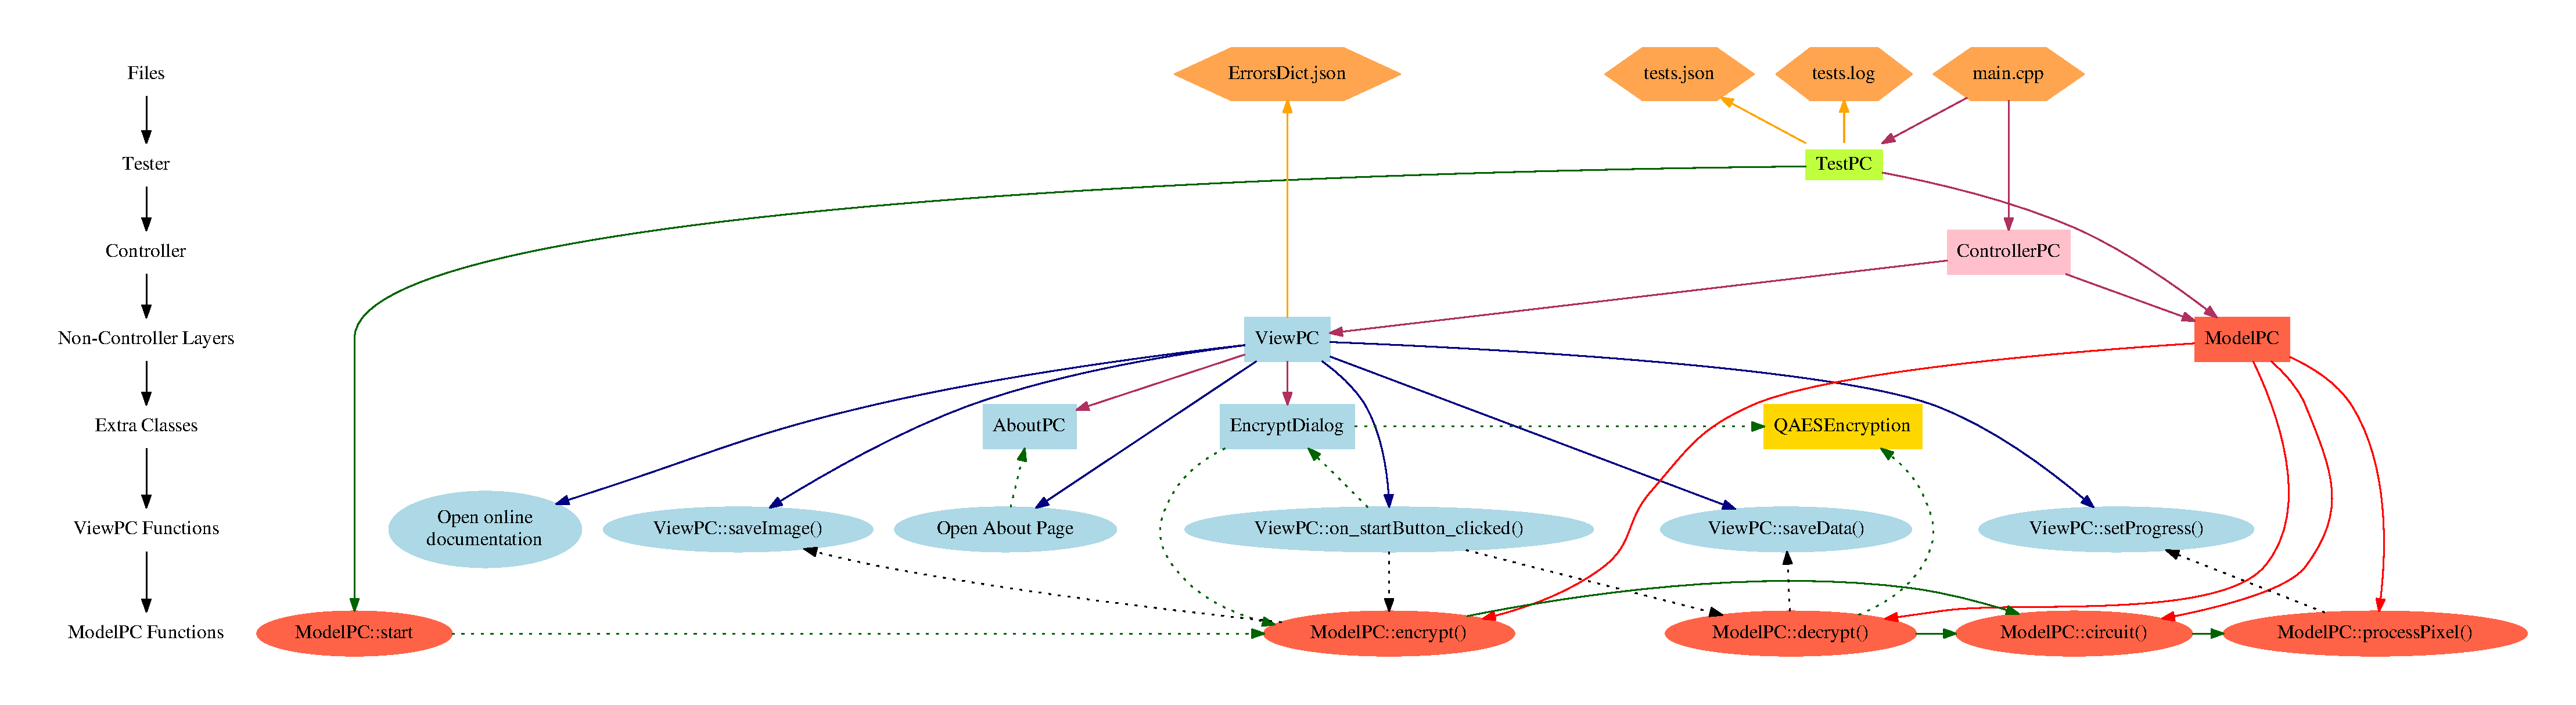
\includegraphics[width=\textwidth,height=\textheight/2,keepaspectratio=true]{dot_mainpage}}
\end{DoxyImageNoCaption}
 Well... I think you didn\textquotesingle{}t quite understand what is happening here... So hop into my \char`\"{}\+User-\/friendly\char`\"{} Documentation!

See source on \href{https://github.com/waleko/PictureCrypt}{\tt https\+://github.\+com/waleko/\+Picture\+Crypt}

\begin{DoxyNote}{Note}
\hyperlink{class_q_a_e_s_encryption}{Q\+A\+E\+S\+Encryption} class done by \href{https://github.com/bricke}{\tt Bricke}
\end{DoxyNote}
\hypertarget{index_ext-use}{}\section{External use}\label{index_ext-use}
\hyperlink{class_model_p_c}{Model\+PC} class can be used externally (without UI) \begin{DoxyNote}{Note}
Test\+PC class was introduced recently, its use is adviced.
\end{DoxyNote}

\begin{DoxyCode}
\textcolor{preprocessor}{#include <\hyperlink{modelpc_8h}{modelpc.h}>}
\textcolor{preprocessor}{#include <testpc.h>}
\textcolor{preprocessor}{#include <QByteArray>}
\textcolor{preprocessor}{#include <QImage>}

\textcolor{preprocessor}{#include <QDebug>} \textcolor{comment}{// Just for demonstration use}

...

if(TestPC::Test())
    \textcolor{keywordflow}{return};
\hyperlink{class_model_p_c}{ModelPC} * model = \textcolor{keyword}{new} \hyperlink{class_model_p_c}{ModelPC}();

\textcolor{comment}{// Embedding}
QImage * resultImage = model->start(QByteArray data, \textcolor{comment}{// Data to be embedded}
                                    QImage *image, \textcolor{comment}{// Image for embedding}
                                    \textcolor{keywordtype}{int} mode = 0, \textcolor{comment}{// Mode of embedding}
                                    QString key = \textcolor{stringliteral}{""}, \textcolor{comment}{// Key for extra-encryption (if empty, key will be
       generated automatically)}
                                    \textcolor{keywordtype}{int} bitsUsed = 8, \textcolor{comment}{// Bits per Byte used (better explaination
       ModelPC::bitsUsed)}
                                    QString *error = \textcolor{keyword}{nullptr}); \textcolor{comment}{// Error output, if everything is ok, error
       will be "ok"}
\textcolor{keywordflow}{if}(*error != \textcolor{stringliteral}{"ok"})
    \textcolor{keywordflow}{return};
\textcolor{comment}{// Note *error is just a code of error (like "muchdata", dictionary of error codes is also available on
       github.}

\textcolor{comment}{// De-embedding}
QByteArray output = model->\hyperlink{class_model_p_c_a5995215a34a1e1f504035715a8013809}{decrypt}(QImage * image, \textcolor{comment}{// Image with hidden data}
                                   QString *\_error = \textcolor{keyword}{nullptr}); \textcolor{comment}{// Error output}
\textcolor{keywordflow}{if}(data == output)
   qDebug() << \textcolor{stringliteral}{"Great success!"};
\textcolor{keywordflow}{else}
   qDebug() << \textcolor{stringliteral}{"Fiasco :("};
\end{DoxyCode}
 \begin{DoxySeeAlso}{See also}
\hyperlink{class_model_p_c}{Model\+PC}, \hyperlink{class_model_p_c_ae12ebe65ec973c02a0de4850a7c1e31c}{Model\+P\+C\+::\+Model\+PC}, \hyperlink{class_model_p_c_a0855107fb0ccc247cd9e893fae9bb08a}{Model\+P\+C\+::save\+Data}, \hyperlink{class_model_p_c_a41f5e2e8022679046e4d3fa1109025fa}{Model\+P\+C\+::save\+Image}, \hyperlink{class_model_p_c_af0217a7ca5671e26090dc50a5dccdaf5}{Model\+P\+C\+::alert\+View}, \hyperlink{class_model_p_c_afdcd80f0ed5062e145a71f09b0897547}{Model\+P\+C\+::set\+Progress}
\end{DoxySeeAlso}
\hypertarget{index_jphs-use}{}\section{J\+P\+H\+S use}\label{index_jphs-use}
The newer versions of the app have jphs support, but they don\textquotesingle{}t have jphs built in as it is provided under G\+NU General Public License v3.\+0, is \char`\"{}for test purposes only\char`\"{} and is illegal in some countries, so... \begin{DoxyAttention}{Attention}
We support J\+P\+HS, but we don\textquotesingle{}t use any responsibility for it, we never used or downloaded it, we just used .exe output in the web, and it somehow works by chance. All responsibility for using jphs is on you, that is why we use made only optionally. That means that to use jphs with our app you will have to download the jphs yourself and specify the jphs directory. However we provide link to the site where you can download the supported version of the jphs\+: \href{http://linux01.gwdg.de/~alatham/stego.html}{\tt http\+://linux01.\+gwdg.\+de/$\sim$alatham/stego.\+html} As it\textquotesingle{}s not our site publishing the dangerous zip file, we just put link to that site (Google does that too, so what? Sue Google?), This text is subject to United Nations\textquotesingle{} Universal Declaration of Human Rights, (see Article 19 \href{http://www.un.org/en/universal-declaration-human-rights}{\tt http\+://www.\+un.\+org/en/universal-\/declaration-\/human-\/rights})\+: \begin{quote}
Everyone has the right to freedom of opinion and expression; this right includes freedom to hold opinions without interference and to seek, receive and impart information and ideas through any media and regardless of frontiers. \end{quote}
And I typed this link randomly, and I\textquotesingle{}m scared...
\end{DoxyAttention}
\hypertarget{index_license}{}\section{License}\label{index_license}
This software is provided under the \href{http://unlicense.org}{\tt U\+N\+L\+I\+C\+E\+N\+SE}\hypertarget{index_contact}{}\section{Contact us}\label{index_contact}
Visit my site\+: \href{https://www.alexkovrigin.me}{\tt https\+://www.\+alexkovrigin.\+me}

Email me at \href{mailto:a.kovrigin0@gmail.com}{\tt a.\+kovrigin0@gmail.\+com}

\begin{DoxyAuthor}{Author}
Alex Kovrigin (waleko) 
\end{DoxyAuthor}
\begin{DoxyCopyright}{Copyright}
Alex Kovrigin 2018  
\end{DoxyCopyright}
